%%%%%%%%%%%%%%%%%%%%%%%%%%%%%%%%%%%%%%%%%%%%%%%%%%%%%%%%%%%%%%%%%%%%%%%%%%%%%%%%
%2345678901234567890123456789012345678901234567890123456789012345678901234567890
%        1         2         3         4         5         6         7         8

\documentclass[letterpaper, 10 pt, conference]{ieeeconf}  % Comment this line out if you need a4paper



%\documentclass[a4paper, 10pt, conference]{ieeeconf}      % Use this line for a4 paper

\IEEEoverridecommandlockouts                              % This command is only needed if 
                                                          % you want to use the \thanks command

\overrideIEEEmargins                                      % Needed to meet printer requirements.

%In case you encounter the following error:
%Error 1010 The PDF file may be corrupt (unable to open PDF file) OR
%Error 1000 An error occurred while parsing a contents stream. Unable to analyze the PDF file.
%This is a known problem with pdfLaTeX conversion filter. The file cannot be opened with acrobat reader
%Please use one of the alternatives below to circumvent this error by uncommenting one or the other
%\pdfobjcompresslevel=0
%\pdfminorversion=4

% See the \addtolength command later in the file to balance the column lengths
% on the last page of the document

% The following packages can be found on http:\\www.ctan.org
%\usepackage{graphics} % for pdf, bitmapped graphics files
%\usepackage{epsfig} % for postscript graphics files
%\usepackage{mathptmx} % assumes new font selection scheme installed
%\usepackage{times} % assumes new font selection scheme installed
\usepackage{amsmath} % assumes amsmath package installed
\usepackage{amssymb}  % assumes amsmath package installed
\usepackage{hyperref}


 \usepackage{easyReview}
 


\title{\LARGE \bf
Matrix Multiplication-Driven Repulsive Fields for 3D Voxel-Based TSDF Calculation
}


\author{
	Jakob Baumgartner$^{1}$ and Gregor Klančar$^{2}$% <-this % stops a space
%\thanks{*This work was not supported by any organization}% <-this % stops a space
%\thanks{$^{1}$Albert Author is with Faculty of Electrical Engineering, Mathematics and Computer Science,
%        University of Twente, 7500 AE Enschede, The Netherlands
%        {\tt\small albert.author@papercept.net}}%
%\thanks{$^{2}$Bernard D. Researcheris with the Department of Electrical Engineering, Wright State University,
%        Dayton, OH 45435, USA
%        {\tt\small b.d.researcher@ieee.org}}%
}


\begin{document}



\maketitle
\thispagestyle{empty}
\pagestyle{empty}


%%%%%%%%%%%%%%%%%%%%%%%%%%%%%%%%%%%%%%%%%%%%%%%%%%%%%%%%%%%%%%%%%%%%%%%%%%%%%%%%
\begin{abstract}



\end{abstract}


%%%%%%%%%%%%%%%%%%%%%%%%%%%%%%%%%%%%%%%%%%%%%%%%%%%%%%%%%%%%%%%%%%%%%%%%%%%%%%%%
\section{INTRODUCTION}

\section{RELATED WORKS}

\section{REPULSIVE FIELD CALCULATION}

The operating environment is modelled by discrete voxels. As the robots environment can dynamically change, we propose a method that looks at the surrounding space of the robot and calculates these direction away from all the surrounding obstacles in real time. We only look in a predefined area / perimeter arround the robot.  

In 3D computer graphics, a voxel represents a value on a regular grid in three-dimensional space. Each of the voxels holds the probability value of its occupation. In case of voxel being empty it holds the value of 0, if the voxel is occupied it holds the value of non-zero, depending on our assurance of it being occupied. If it is definitly occupied it holds the value of 1. 

Mreža voxels je lahko predefinirana, glede na model / 3d zemljevid prostora. Zasedenost voxlov lahko spreminjamo glede na poznane pozicije in trajektorije preostalih agentov v prostoru. Kot omenjeno v uvodu, pa lahko zasedenost voxlov pridobimo tudi z senzorskimi sistemi. 

In our method, we compute repulsive velocities within the task space using a novel matrix kernel multiplication approach. Concentrating on the task space is advantageous as it provides a more direct and realistic representation of the environment. 

Naša metoda je posebno primerna za uporabo z senzorskimi sistemi kot so LIDAR ali globinske kamere, saj zaradi upoštevanja celotne okolice točke in ne le razdalje do najbližje točke v okolici efektivno filtriramo senzorski šum.

Repulsive velocities tell the agent in which direction to move, so that it avoids nearby obstacles. These velocities drop to zero when the agent maintains a minimum safe distance from obstacles, and rise to their highest when it nears an obstacle, facilitating immediate evasive action. As the repulsive field calculation is locally based, it will also go to zero when the agent is surrounded by all directions, equally spaced from all sides. That is, it is in the best local minima away from all the obstacles. 

\subsection{MAPPING}

Since the obstacle space is discrete (has finite resolution), while the Cartesian space is continuous, we propose two methods for mapping from Cartesian space to the occupancy grid space. The simpler approach involves mapping the point directly to the center of the nearest occupancy grid voxel, based on Euclidean distance.\add{is this clear, do i need equation?} However, this discretization can sometimes lead to discontinuities. Therefore, we propose a second approach: tri-linear interpolation of the calculated repulsive field to achieve a continuous repulsive field value.

Once the mapping of these points to the voxel grid is completed, we proceed to employ a specialized kernel convolution method. This method is tailored to calculate the components of the avoidance velocity vector in the Cartesian space, we generate the corresponding kernel and extract a segment of the obstacle grid of matching size, centered at agent or the point of interest (POI), resulting in two same size 3D matrices—one is a "window" from the obstacle grid $A_d$ and the other representing the kernel $K_d$.

If the agent is located near the edge of our known voxel grid we can set the eleemnts of the window would be located in the space beyond the matrix as empty in which case the robot might want to move towards this space or as occupied, which will prevent the robot from moving out of the known grid space.

By employing the Hadamard (element-wise) product (eq.~\ref{eq:hadamard}) between the cutout segment of the obstacle grid \(A_d\) and the corresponding 3D convolutional kernel \(K_d\) for direction \(d\), we derive the resultant matrix \(C_d\), which can be expressed as:

%\begin{equation}
%	C_d = A_d \odot K_d
%	\label{eq:hadamard}
%\end{equation}

\begin{equation}
	S = \sum_{i,j,k} (W \odot A)_{ijk} = \sum_{i}\sum_{j}\sum_{k} w_{\Delta i \Delta j \Delta k} \times  a_{\Delta i \Delta j \Delta k}
\end{equation}

Subsequently, the avoidance velocity in the Cartesian coordinate system is obtained (eq.~\ref{eq:summation}) by summing all the values in the resulting matrix $C_d$, which can be represented as:

\begin{equation}
	\dot{x}_{poi} = \sum_{i}\sum_{j}\sum_{k} c_{dijk} 
	\label{eq:summation}
\end{equation}

\alert{remove the above equation and add a vector of calculated velocities equation instead}

\comment{}{TODO: add the indexes for x,y,z directions}



\subsection{KERNELS SELECTION}

The fundamental concept of our directional kernels lies in computing the repulsive field individually for each direction within the Cartesian coordinate system. \remove{Our filters structure was inspired by the Sobel  operator, a 2D convolutional filter frequently utilized in computer vision for calculating image gradients at specific points.}

Our kernels are designed as three-dimensional matrixes with a primary kernel axis aligned along a specific Cartesian direction, corresponding to the calculated repulsive velocity. The two secondary kernel axes are orthogonal to this primary axis. The distribution of values along the primary axis is inversely symmetric, exhibiting positive values on one side and negative values on the other, with the zero valued cell in the center of the kernel, where jump between max positive and max negative magnitude is. The function of the increase in magnitude along the primary axis of the kernel defines the shape of the repulsive velocity field, determining how the repulsive velocity changes as the agent approaches an obstacle. Moreover, it is essential for the magnitudes at the kernel's periphery to be minimal, promoting a smooth increase in repulsive velocity when approaching the obstacle rather than a sudden spike.

% KERNEL WEIGHTS

% PRIMARY AXIS

We propose two different primary axis weights distributions, of course there is no reason why any other distribution of weights could not be used. The choice of the weights distribution should depend on the profile of the repulsive velocities we want to archieve for the APF. 

The first of the proposed functions is a mirrored normal / gaussian distribution. By changing the sigma we can control how fast or slow does the field value grow when we approach obstacles.

$\Delta i = c_i - i$, $\Delta j = c_j - j$ in $\Delta k = c_k - k$ predstavljajo število celic odmika od centralnega polja matrike, v katerem se nahaja naša točka na agentu v posamezno koordinatno smer.

\begin{equation}
w_{\Delta i} = 
\begin{cases} 
	e^{-\frac{\Delta i^2}{2\sigma^2}} / (\sigma \sqrt{2\pi}) & \text{if } \Delta i > 0 \\
	0 & \text{if } \Delta i = 0 \\
	-e^{-\frac{\Delta i^2}{2\sigma^2}} / (\sigma \sqrt{2\pi}) & \text{if } \Delta i < 0 
\end{cases}
\end{equation}

%\begin{equation}
%w_i = 
%\begin{cases} 
%	\frac{e^{-\frac{\Delta i^2}{2\sigma^2}}}{\sigma \sqrt{2\pi}} & \text{if } \Delta i > 0 \\
%	0 & \text{if } \Delta i = 0 \\
%	-\frac{e^{-\frac{\Delta i^2}{2\sigma^2}}}{\sigma \sqrt{2\pi}} & \text{if } \Delta i < 0 
%\end{cases}
%\end{equation}

Another distribution we used is mirrored linear, where the $l=\lfloor width / 2 \rfloor$ is the rounded down half length of the primary axis kernel. 

\begin{equation}
	w_{\Delta i} = 
	\begin{cases} 
	 	\frac{l - \Delta i}{l} & \text{if } \Delta i > 0 \\
		0 & \text{if } \Delta i = 0 \\
		\frac{l + \Delta i}{l}& \text{if } \Delta i < 0 
	\end{cases}
\end{equation}

% ORTHAGONAL AXIS

If the matrix would be only 1 field width and height the field would work kind of as ray tracing in each of the main cartesian coordinate directions. Since our need is to detect also obstacles that dont align perfectly along the cartesian direction, it is important that our matrixes have width and height. However as we want bigger repulsive field when the obstacle is head on in the direction than when the obstacle is off the cardinal direction, we propose the following multiplicator, to account for the off direction obstacles.




The length of the primary axis is critical, as it dictates the detection range for obstacles. Longer kernels can detect obstacles further away
from the robot, essentially extending the ’safety zone’ around the robot. If the primary axis is too long, it can lead to extra calculations and may cause the robot to unnecessarily avoid obstacles that aren't in its immediate path, making its movement and path planning less efficient. A kernel with a primary axis that is too short might restrict the robot's ability to maneuver, detecting obstacles potentially too late, compromising the robots capacity to avoid obstacles effectively (eq. \ref{eq: detect range}). 

\begin{equation}
	\label{eq: detect range}
	num_{primary} = \frac{2 \times \mathrm{range}}{\Delta \mathrm{grid}}\\
\end{equation}

\add{mogoče dodaj še kak stavek o izbiri dimenzij matrik}

%\remove{In the orthogonal axes, the magnitude of values diminishes with increasing distance from the core of the kernel, nearing zero at the edges. This gradation is vital for a smooth velocity transition when obstacles emerge in the kernels range. The peak magnitude is located at the kernel's core, along the primary axis. The polarity of the values is determined by their position relative to the primary axis. }

The length of the orthogonal axes influences the peripheral detection range for obstacles. Excessively wide kernels may generate repulsive velocities for objects that are not in the path of the robot, whereas too narrow kernels might only detect obstacles aligned directly with the Cartesian direction in the point of interest. When selecting the width and height of the kernel, we must consider the density of the neighboring points of interest on the agent, ensuring that the \replace{collective fields}{combination of kernels} adequately cover the entire agent's surrounding area. 

For smooth transitions when approaching the obstacles we propose the following sinus based function for the orthagonal axis distributions. The proposed equation is the same for both of the orthagonal matrix directions / axis. That is of course while operating with axis the $r=\lfloor width / 2 \rfloor$ is the rounded down half length of the selected orthagonal axis kernel.

\begin{equation}
	w_{\Delta j} =
	\begin{cases} 
		sin(\left| \Delta j \right| \pi / (2 r)) & \text{if } \Delta j < 0 \text{~or }  \Delta j > 0 \\
		1 & \text{if } \Delta j = 0 \\
	\end{cases}
\end{equation}

Another option is to use linearly falling weights.

\begin{equation}
	w_{\Delta j} =
	\begin{cases} 
		\frac{l - \Delta j }{l} & \text{if } \Delta j < 0 \text{~or }  \Delta j > 0 \\
		1 & \text{if } \Delta j = 0 \\
	\end{cases}
\end{equation}


Finally we get three matrix kernels, one for each of the three coordinate axis directions by multiplieing weights components for primary and orthagonal axis.

\begin{equation}
	w_{\Delta i \Delta j \Delta k} = w_{\Delta i} * w_{\Delta j} * w_{\Delta k}
\end{equation}

Če imamo opravka s točkastim agentom, kot je recimo štirikopet - dron, potem je dobra oblika posameznih matrik enaka dimenzija dolžine, širine in višine. Tako dobimo enakomerno pokritost krogle prostora v okolici agenta in preprečimo mrtve kote, ki se sicer lahko pojavijo, ko se ovira nahaja v bližini agenta, vendar med posameznimi jedri. \add{ADD:primer,slika}

\comment{}{PLOT: kernel 2D images}
\comment{}{EQUATION: kernel generation / values equations}





\subsection{3D INTERPOLATION} 


It is essential that the velocity contributions affecting the robot change smoothly. However, since our obstacle grid is discretely defined, achieving perfect continuity can be challenging. Increasing the resolution of the obstacle field can theoretically bring us closer to continuous behavior, but in practice, we are constrained by finite resolution. To ensure that the velocity remains continuous when transitioning from one cell of the obstacle grid to another at a point of interest (POI), we employ trilinear interpolation. \remove{This technique allows for a smooth and continuous linear approximation of velocities in all three Cartesian directions (x, y, and z) as the POI moves between cells.}

We start by scalling the coordinates of POI into the grid koordinate system, by multiplying it by grid resolution (eq.~\ref{eq:scale grid}). 

\begin{equation}
	\label{eq:scale grid}
	\vec{P} = \vec{p}_{\mathrm{POI}} \times\Delta \mathrm{grid}
\end{equation}

We get the indexes of the surrounding cells by first scaling the POI position by grid resolution and than rounding the position to the nearest lower and upper integer positions (eq.~\ref{eq:floor and ceil}).

%\begin{equation}
% X = \left[ \lfloor p_{x} \rfloor, \lceil p_{x} \rceil \right] 
%\end{equation}
%
%\begin{equation}
% Y = \left[ \lfloor p_{y} \rfloor, \lceil p_{y} \rceil \right] 
%\end{equation}
%
% \begin{equation}
% Z = \left[ \lfloor p_{z} \rfloor, \lceil p_{z} \rceil \right] 
%\end{equation}

\begin{equation}
	\label{eq:floor and ceil}
	\vec{P} =
	\begin{bmatrix}
		X \\
		Y \\
		Z \\
	\end{bmatrix}
	=
	\begin{bmatrix}
		\; \lfloor \vec{p}_{\mathrm{POI}}(1) \rfloor \; \lceil \vec{p}_{\mathrm{POI}}(1) \rceil \;  \\
		\; \lfloor \vec{p}_{\mathrm{POI}}(2) \rfloor \; \lceil \vec{p}_{\mathrm{POI}}(2) \rceil \; \\
		\; \lfloor \vec{p}_{\mathrm{POI}}(3) \rfloor \; \lceil \vec{p}_{\mathrm{POI}}(3) \rceil \; 
	\end{bmatrix}
\end{equation}

Once we got the indexes of the eight surrounding cells of our POI, we use our kernel matrix multiplication method, to calculate the 3x1 repulsive velocity vectors for all the cells (eq.~\ref{eq: calc rep vel}).

\begin{equation}
	\label{eq: calc rep vel}
	\vec{V}rep_{xyz,ijk} = \mathrm{calc\_rep\_vel}(X[i], Y[j], Z[k]) \quad \forall i, j, k \in \{1, 2\}
\end{equation}

Trilinear interpolation method works on a 3-dimensional regular grid. Before we can start with the interpolation we need to calculate the distance between POI and smaller coordinates of the cells where we calculated the repulsive velocities (eq.~\ref{eq: deltas interp}). \replace{Since the repulsive values we calculate for the cells are alligned with the centers of the cells, we need to move before the interpolation the positions of known grid points by half of the cell width.}{The calculated repulsive velocity values are located at the centers of the cells. Therefore, before interpolation, we shift the values of the cells coordinates by half the resolution of the obstacle grid for each direction. }

%\begin{equation}
%	\Delta X = \frac{\left( P_x - \left( X(1) + \frac{1}{2} \Delta \mathrm{grid} \right)  \right)}{\left( X(2) - X(1) \right)}
%\end{equation}
%
%\begin{equation}
%	\Delta Y = \frac{\left( P_y - \left( Y(1) + \frac{1}{2} \Delta \mathrm{grid} \right)  \right)}{\left( Y(2) - Y(1) \right)}
%\end{equation}
%
%\begin{equation}
%	\Delta Z = \frac{\left( P_z - \left( Z(1) + \frac{1}{2} \Delta \mathrm{grid} \right)  \right)}{\left( Z(2) - Z(1) \right)}
%\end{equation}

\begin{equation}
	\label{eq: deltas interp}
	\Delta \vec{P} =
	\begin{bmatrix}
		\Delta x \\
		\Delta y \\
		\Delta z		
	\end{bmatrix}
	=
	\begin{bmatrix}
		\frac{\left( P_x - \left( X(1) + \frac{1}{2} \Delta \mathrm{grid} \right)  \right)}{\left( X(2) - X(1) \right)} \\
		\frac{\left( P_y - \left( Y(1) + \frac{1}{2} \Delta \mathrm{grid} \right)  \right)}{\left( Y(2) - Y(1) \right)} \\
		\frac{\left( P_z - \left( Z(1) + \frac{1}{2} \Delta \mathrm{grid} \right)  \right)}{\left( Z(2) - Z(1) \right)} \\
	\end{bmatrix}
\end{equation}

The result of the interpolation is independent of the order of the operations. We first interpolate along the x-axis, followed by along the y-axis and finally along z-axis.

%\begin{equation}
%	\vec{V}_{rep,00} = \vec{V}_{rep,000}(1 - x_d) + \vec{V}_{rep,100}x_d
%\end{equation}
%\begin{equation}
%	\vec{V}_{rep,01} = \vec{V}_{rep,001}(1 - x_d) + \vec{V}_{rep,101}x_d
%\end{equation}
%\begin{equation}
%	\vec{V}_{rep,10} = \vec{V}_{rep,010}(1 - x_d) + \vec{V}_{rep,110}x_d
%\end{equation}
%\begin{equation}
%	\vec{V}_{rep,11} = \vec{V}_{rep,011}(1 - x_d) + \vec{V}_{rep,111}x_d
%\end{equation}
	
\begin{equation}
	\label{eq: interp x}
	\vec{V}rep_{xyz,jk} = \vec{V}rep_{xyz,0jk}(1 - \Delta x) + \vec{V}rep_{xyz,1jk} \, \Delta x \quad \forall \, j, k \in \{1, 2\}
\end{equation}

%\begin{equation}
%	\vec{V}rep_{xyz,0} = \vec{V}rep_{xyz,00}(1 - \Delta y) + \vec{V}rep_{xyz,10} \, \Delta y
%\end{equation}
%
%\begin{equation}
%	\vec{V}rep_{xyz,1} = \vec{V}rep_{xyz,01}(1 - \Delta y) + \vec{V}rep_{xyz,11} \, \Delta y
%\end{equation}

\begin{equation}
	\label{eq: interp y}
	\vec{V}rep_{xyz,k} = \vec{V}rep_{xyz,0k}(1 - \Delta y) + \vec{V}rep_{xyz,1k} \, \Delta y \quad \forall \, k \in \{1, 2\}
\end{equation}

\begin{equation}
	\label{eq: interp z}
	\vec{V}rep_{xyz} = \vec{V}rep_{xyz,0}(1 - \Delta z) + \vec{V}rep_{xyz,1} \, \Delta z 
\end{equation}

The final result is a repulsive velocity vector that transitions smoothly between the discrete values calculated at distinct points in the obstacle grid.

\section{SIMULATION RESULTS}

\subsection{Repulsive Field Visualization}

\add{Visualization of the repulsive field around more or less complicated obstacles.}

\begin{figure}[h]
	\centering
	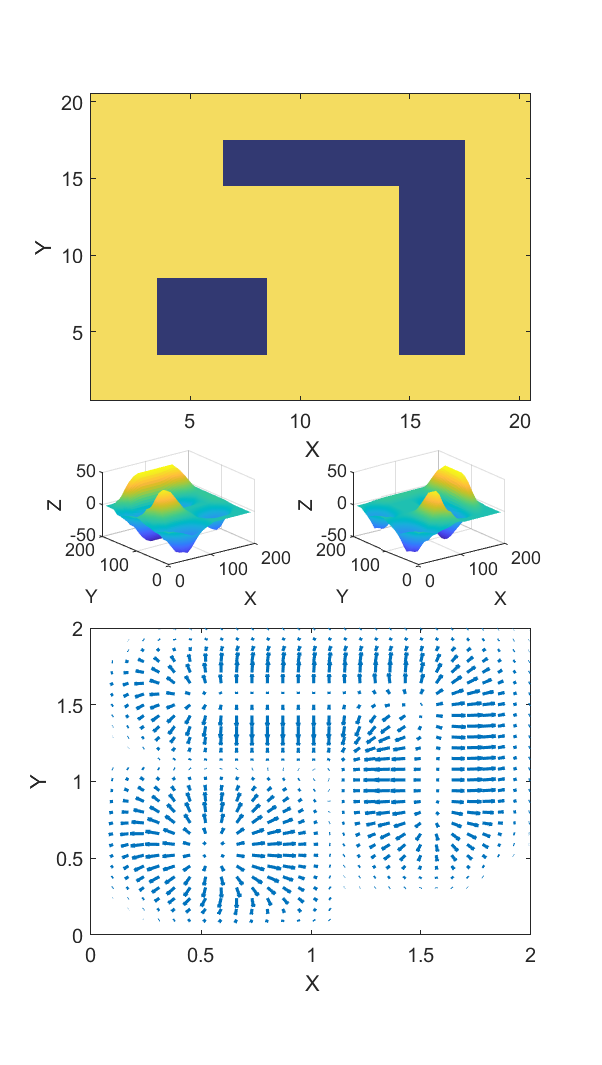
\includegraphics[width=0.95\linewidth]{demo-field1.eps} % Replace 'example-image' with the filename of your image
	\caption{Example Image}
	\label{fig:example-field}
\end{figure}

\add{add label, caption, every plot has different axis scale}

\comment{}{we dont have the close obstacles bottlenecks, we do have weird bottlenecks in the orthagonal directions - maybe}

\subsection{Repulsive Field Interpolation}

\begin{figure}[h]
	\centering
	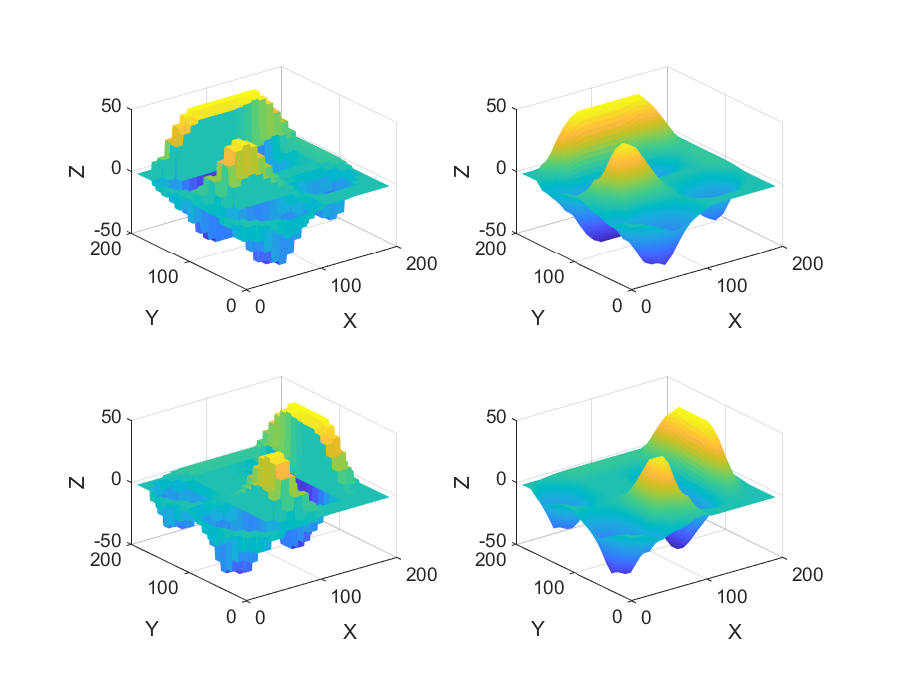
\includegraphics[width=1\linewidth]{non_and_interp_4_plots.eps} % Replace 'example-image' with the filename of your image
	\caption{Example Image}
	\label{fig:interp-experiment}
\end{figure}

\subsection{Manipulator Examples}

\add{EXAMPLE: MANIPULATOR AND COLUMN}

\add{EXAMPLE: MANIPULATOR AND MOVING NOISY BALL}

\remove{Drone Example}

\remove{EXAMPLE: DRONE MOVING THROUGH THE MAP OF OBSTACLES USING APF}

\section{CONCLUSION}

\addtolength{\textheight}{-12cm}   % This command serves to balance the column lengths
                                  % on the last page of the document manually. It shortens
                                  % the textheight of the last page by a suitable amount.
                                  % This command does not take effect until the next page
                                  % so it should come on the page before the last. Make
                                  % sure that you do not shorten the textheight too much.


\begin{thebibliography}{99}
	
\bibitem{IDEASLab2023}
IDEAS Lab, "Motion and Path Planning," presented at Purdue University, 2023. [Online]. Available: \url{https://ideas.cs.purdue.edu/research/robotics/planning/}. Accessed on: Jan. 9, 2024.
	
\bibitem{c21} E. A. Basso and K. Y. Pettersen, “Task-Priority Control of Redundant Robotic Systems using Control Lyapunov and Control Barrier Function based Quadratic Programs,” in IFAC-PapersOnLine, vol. 53, no. 2, pp. 9037–9044, 2020. doi: 10.1016/j.ifacol.2020.12.2024.


\bibitem{c22} H. Toshani and M. Farrokhi, “Real-time inverse kinematics of redundant manipulators using neural networks and quadratic programming: A Lyapunov-based approach,” Robotics and Autonomous Systems, vol. 62, no. 6, pp. 766–781, Jun. 2014. doi: 10.1016/j.robot.2014.02.005.

\bibitem{haviland2021neo} J. Haviland and P. Corke, “NEO: A Novel Expeditious Optimisation Algorithm for Reactive Motion Control of Manipulators,” IEEE Robot. Autom. Lett., vol. 6, no. 2, Art. no. 2, Apr. 2021, doi: 10.1109/LRA.2021.3056060.


\bibitem{c23} Y. Zhang, S. S. Ge, and T. H. Lee, “A Unified Quadratic-Programming-Based Dynamical System Approach to Joint Torque Optimization of Physically Constrained Redundant Manipulators,” IEEE Trans. Syst., Man, Cybern. B, vol. 34, no. 5, pp. 2126–2132, Oct. 2004. doi: 10.1109/TSMCB.2004.830347.

\bibitem{c24} J. Nakanishi, R. Cory, M. Mistry, J. Peters, and S. Schaal, “Comparative experiments on task space control with redundancy resolution,” in Proc. 2005 IEEE/RSJ Int. Conf. on Intelligent Robots and Systems, Edmonton, Alta., Canada, 2005, pp. 3901–3908. doi: 10.1109/IROS.2005.1545203.

\bibitem{c25} M. H. Raibert and J. J. Craig, “Hybrid Position/Force Control of Manipulators,” Journal of Dynamic Systems, Measurement, and Control, vol. 103, no. 2, pp. 126–133, Jun. 1981. doi: 10.1115/1.3139652.

\bibitem{c26} T. Yoshikawa, “Dynamic hybrid position/force control of robot manipulators--Description of hand constraints and calculation of joint driving force,” IEEE J. Robot. Automat., vol. 3, no. 5, pp. 386–392, Oct. 1987. doi: 10.1109/JRA.1987.1087120.

\bibitem{c27} O. Khatib, “A unified approach for motion and force control of robot manipulators: The operational space formulation,” IEEE J. Robot. Automat., vol. 3, no. 1, pp. 43–53, Feb. 1987. doi: 10.1109/JRA.1987.1087068.

\bibitem{c28} N. Hogan, “Impedance Control: An Approach to Manipulation,” in Proc. 1984 American Control Conf., San Diego, CA, USA, Jul. 1984, pp. 304–313. doi: 10.23919/ACC.1984.4788393.

\bibitem{c29} A. A. Maciejewski and C. A. Klein, “Obstacle Avoidance for Kinematically Redundant Manipulators in Dynamically Varying Environments,” The International Journal of Robotics Research, vol. 4, no. 3, pp. 109–117, Sep. 1985. doi: 10.1177/027836498500400308.

\bibitem{c30} L. Lajpah and T. Petri, “Obstacle Avoidance for Redundant Manipulators as Control Problem,” in Serial and Parallel Robot Manipulators - Kinematics, Dynamics, Control and Optimization, S. Kucuk, Ed. InTech, 2012. doi: 10.5772/32651.

\bibitem{c31} R. Colbaugh and K. Glass, “Cartesian control of redundant robots,” J. Robotic Syst., vol. 6, no. 4, pp. 427–459, Aug. 1989. doi: 10.1002/rob.4620060409.

\bibitem{c32} K. Glass, R. Colbaugh, D. Lim, and H. Seraji, “Real-time collision avoidance for redundant manipulators,” IEEE Trans. Robot. Automat., vol. 11, no. 3, pp. 448–457, Jun. 1995. doi: 10.1109/70.388789.

\bibitem{c33} O. Khatib, “Real-time obstacle avoidance for manipulators and mobile robots,” in 1985 IEEE International Conference on Robotics and Automation Proceedings, Mar. 1985, pp. 500–505. doi: 10.1109/ROBOT.1985.1087247.

\bibitem{c34} L. Sciavicco and B. Siciliano, “A solution algorithm to the inverse kinematic problem for redundant manipulators,” IEEE J. Robot. Automat., vol. 4, no. 4, pp. 403–410, Aug. 1988. doi: 10.1109/56.804.

\bibitem{c35} L. Sciavicco and B. Siciliano, “Solving the Inverse Kinematic Problem for Robotic Manipulators,” in RoManSy 6, A. Morecki, G. Bianchi, and K. Kedzior, Eds., Boston, MA: Springer US, 1987, pp. 107–114. doi: 10.1007/978-1-4684-6915-8\_9.

\bibitem{c36} O. Egeland, “Task-space tracking with redundant manipulators,” IEEE J. Robot. Automat., vol. 3, no. 5, pp. 471–475, Oct. 1987. doi: 10.1109/JRA.1987.1087118.

\bibitem{c37} H. Seraji, “Configuration control of redundant manipulators: theory and implementation,” IEEE Trans. Robot. Automat., vol. 5, no. 4, pp. 472–490, Aug. 1989. doi: 10.1109/70.88062.

\bibitem{c38} Y. Nakamura, H. Hanafusa, and T. Yoshikawa, “Task-Priority Based Redundancy Control of Robot Manipulators,” The International Journal of Robotics Research, vol. 6, no. 2, pp. 3–15, Jun. 1987. doi: 10.1177/027836498700600201.

\bibitem{c39} B. Siciliano and O. Khatib, Eds., Springer Handbook of Robotics. in Springer Handbooks. Cham: Springer International Publishing, 2016. doi: 10.1007/978-3-319-32552-1.

\bibitem{c40} J.-O. Kim and P. Khosla, “Real-Time Obstacle Avoidance Using Harmonic Potential Functions,” 1992. doi: 10.1109/70.143352.

\bibitem{c41} L. Zlajpah and B. Nemec, “Kinematic control algorithms for on-line obstacle avoidance for redundant manipulators,” in Proc. IEEE/RSJ International Conference on Intelligent Robots and Systems, Lausanne, Switzerland, 2002, pp. 1898–1903. doi: 10.1109/IRDS.2002.1044033.

\bibitem{c42} T. Petrič and L. Žlajpah, “Smooth continuous transition between tasks on a kinematic control level: Obstacle avoidance as a control problem,” Robotics and Autonomous Systems, vol. 61, no. 9, Art. no. 9, Sep. 2013. doi: 10.1016/j.robot.2013.04.019.

\bibitem{c43} M. F. Pinto, T. R. F. Mendonça, L. R. Olivi, E. B. Costa, and A. L. M. Marcato, “Modified approach using variable charges to solve inherent limitations of potential fields method,” in Proc. 2014 11th IEEE/IAS International Conference on Industry Applications, Dec. 2014, pp. 1–6. doi: 10.1109/INDUSCON.2014.7059414.

\bibitem{c44} Z. Long, “Virtual target point-based obstacle-avoidance method for manipulator systems in a cluttered environment,” Engineering Optimization, vol. 52, no. 11, Art. no. 11, Nov. 2020. doi: 10.1080/0305215X.2019.1681986.

\bibitem{c45} A. H. Qureshi and Y. Ayaz, “Potential Functions based Sampling Heuristic For Optimal Path Planning,” Auton Robot, vol. 40, no. 6, Art. no. 6, Aug. 2016. doi: 10.1007/s10514-015-9518-0.

\bibitem{c46} A. H. Qureshi et al., “Adaptive Potential guided directional-RRT*,” in Proc. 2013 IEEE International Conference on Robotics and Biomimetics (ROBIO), Shenzhen, China, Dec. 2013, pp. 1887–1892. doi: 10.1109/ROBIO.2013.6739744.

\bibitem{c47} J. Yi, Q. Yuan, R. Sun, and H. Bai, “Path planning of a manipulator based on an improved P\_RRT* algorithm,” Complex Intell. Syst., vol. 8, no. 3, pp. 2227–2245, Jun. 2022. doi: 10.1007/s40747-021-00628-y.

\bibitem{c48} T. Zhu, J. Mao, L. Han, C. Zhang, and J. Yang, “Real-Time Dynamic Obstacle Avoidance for Robot Manipulators Based on Cascaded Nonlinear MPC With Artificial Potential Field,” IEEE Trans. Ind. Electron., pp. 1–11, 2023. doi: 10.1109/TIE.2023.3306405.

\bibitem{c49} X. Xia et al., “Path Planning for Obstacle Avoidance of Robot Arm Based on Improved Potential Field Method,” Sensors, vol. 23, no. 7, Art. no. 7, Apr. 2023. doi: 10.3390/s23073754.

\bibitem{c50} Y. Chen, L. Chen, J. Ding, and Y. Liu, “Research on Real-Time Obstacle Avoidance Motion Planning of Industrial Robotic Arm Based on Artificial Potential Field Method in Joint Space,” Applied Sciences, vol. 13, no. 12, p. 6973, Jan. 2023. doi: 10.3390/app13126973.

\bibitem{c51} S. M. LaValle, Planning Algorithms. Cambridge: Cambridge University Press, 2006.

\bibitem{c52} M. G. Tamizi, M. Yaghoubi, and H. Najjaran, “A review of recent trend in motion planning of industrial robots,” Int J Intell Robot Appl, vol. 7, no. 2, Art. no. 2, Jun. 2023. doi: 10.1007/s41315-023-00274-2.

\bibitem{vsvestka1997motion} P. {\v{S}}vestka and M. H. Overmars, “Motion planning for carlike robots using a probabilistic learning approach,” The International Journal of Robotics Research, vol. 16, no. 2, pp. 119–143, 1997.

\bibitem{lavalle1998rapidly} S. LaValle, “Rapidly-exploring random trees: A new tool for path planning,” Research Report 9811, 1998.

\bibitem{gammell2015batch} J. D. Gammell, S. S. Srinivasa, and T. D. Barfoot, “Batch Informed Trees (BIT*): Sampling-based Optimal Planning via the Heuristically Guided Search of Implicit Random Geometric Graphs,” in Proc. of the 2015 IEEE International Conference on Robotics and Automation (ICRA), May 2015, pp. 3067–3074. doi: 10.1109/ICRA.2015.7139620.

\bibitem{karaman2010incremental} S. Karaman and E. Frazzoli, "Incremental sampling-based algorithms for optimal motion planning," in Proc. Robotics: Science and Systems (RSS), 2010.

\bibitem{gammell2014informed} J. D. Gammell, S. S. Srinivasa, and T. D. Barfoot, “Informed RRT*: Optimal sampling-based path planning focused via direct sampling of an admissible ellipsoidal heuristic,” in Proc. of the 2014 IEEE/RSJ International Conference on Intelligent Robots and Systems, Chicago, IL, USA, Sep. 2014, pp. 2997–3004. doi: 10.1109/IROS.2014.6942976.

\bibitem{kuffner2000rrt} J. J. Kuffner and S. M. LaValle, “RRT-connect: An efficient approach to single-query path planning,” in Proceedings of the 2000 ICRA. Millennium Conference. IEEE International Conference on Robotics and Automation. Symposia Proceedings (Cat. No.00CH37065), Apr. 2000, pp. 995–1001 vol.2. doi: 10.1109/ROBOT.2000.844730.

\bibitem{siciliano1990kinematic} B. Siciliano, “Kinematic control of redundant robot manipulators: A tutorial,” J. Intell. Robot. Syst., vol. 3, no. 3, Art. no. 3, 1990, doi: 10.1007/BF00126069.

\bibitem{siciliano2016springer} B. Siciliano and O. Khatib, Eds., Springer Handbook of Robotics, in Springer Handbooks. Cham: Springer International Publishing, 2016. doi: 10.1007/978-3-319-32552-1.

\bibitem{siciliano2010robot} B. Siciliano, L. Sciavicco, L. Villani, and G. Oriolo, Robot. Model. Plan. Control, 2010, pp. 161–189. [Online]. Available: http://link.springer.com/10.1007/978-1-84628-642-1\_4

\bibitem{dai2022review} Y. Dai, C. Xiang, Y. Zhang, Y. Jiang, W. Qu, and Q. Zhang, “A Review of Spatial Robotic Arm Trajectory Planning,” Aerospace, vol. 9, p. 361, Jul. 2022, doi: 10.3390/aerospace9070361.

\bibitem{gottschalk1996obbtree} S. Gottschalk, M. C. Lin, and D. Manocha, “OBBTree: a hierarchical structure for rapid interference detection,” in Proceedings of the 23rd Annual Conference on Computer Graphics and Interactive Techniques, ACM, Aug. 1996, pp. 171–180. doi: 10.1145/237170.237244.

\bibitem{vandenbergen1997efficient} G. van den Bergen, “Efficient Collision Detection of Complex Deformable Models using AABB Trees,” Journal of Graphics Tools, vol. 2, no. 4, pp. 1–13, 1997. doi: 10.1080/10867651.1997.10487480.

\bibitem{chen2018path} G. Chen, D. Liu, Y. Wang, Q. Jia, and X. Zhang, “Path planning method with obstacle avoidance for manipulators in dynamic environment,” International Journal of Advanced Robotic Systems, vol. 15, no. 6, Art. no. 1729881418820223, Nov. 2018, doi: 10.1177/1729881418820223.

\bibitem{puiu2011realtime} D. Puiu and F. Moldoveanu, “Real-time collision avoidance for redundant manipulators,” in Proc. of the 2011 6th IEEE International Symposium on Applied Computational Intelligence and Informatics (SACI), Timisoara, Romania, 2011, pp. 403–408, doi: 10.1109/SACI.2011.5873037.

\bibitem{oleynikova2017voxblox} H. Oleynikova, Z. Taylor, M. Fehr, R. Siegwart, and J. Nieto, “Voxblox: Incremental 3D Euclidean Signed Distance Fields for on-board MAV planning,” in Proc. of the 2017 IEEE/RSJ International Conference on Intelligent Robots and Systems (IROS), Vancouver, BC, Sep. 2017, pp. 1366–1373. doi: 10.1109/IROS.2017.8202315.

\bibitem{wurmOctoMap} K. M. Wurm, A. Hornung, M. Bennewitz, C. Stachniss, and W. Burgard, “OctoMap: A Probabilistic, Flexible, and Compact 3D Map Representation for Robotic Systems,” [Details of publication, e.g., in Proc. of the Conference/Journal Name, Year, pp. Page numbers]. [DOI or URL if available].

\bibitem{gao2019flying} F. Gao, W. Wu, W. Gao, and S. Shen, “Flying on point clouds: Online trajectory generation and autonomous navigation for quadrotors in cluttered environments,” Journal of Field Robotics, vol. 36, no. 4, pp. 710–733, 2019, doi: 10.1002/rob.21842.

\bibitem{elfes1989using} A. Elfes, “Using occupancy grids for mobile robot perception and navigation,” Computer, vol. 22, no. 6, pp. 46–57, Jun. 1989, doi: 10.1109/2.30720.

\bibitem{han2019fiesta} L. Han, F. Gao, B. Zhou, and S. Shen, “FIESTA: Fast Incremental Euclidean Distance Fields for Online Motion Planning of Aerial Robots,” arXiv, Jul. 26, 2019. Accessed: Jan. 11, 2024. [Online]. Available: http://arxiv.org/abs/1903.02144

\bibitem{xu2021voxel} Y. Xu, X. Tong, and U. Stilla, “Voxel-based representation of 3D point clouds: Methods, applications, and its potential use in the construction industry,” Automation in Construction, vol. 126, p. 103675, Jun. 2021, doi: 10.1016/j.autcon.2021.103675.

\bibitem{niessner2013realtime} M. Nießner, M. Zollhöfer, S. Izadi, and M. Stamminger, “Real-time 3D reconstruction at scale using voxel hashing,” ACM Trans. Graph., vol. 32, no. 6, pp. 1–11, Nov. 2013, doi: 10.1145/2508363.2508374.

\bibitem{dryanovski2010multivolume} I. Dryanovski, W. Morris, and J. Xiao, “Multi-volume occupancy grids: An efficient probabilistic 3D mapping model for micro aerial vehicles,” in Proc. of the 2010 IEEE/RSJ International Conference on Intelligent Robots and Systems, Taipei, Oct. 2010, pp. 1553–1559. doi: 10.1109/IROS.2010.5652494.

\bibitem{thrun2002probabilistic} S. Thrun, Probabilistic robotics, vol. 45, 2002. Accessed: Jun. 14, 2023. [Online]. Available: https://dl.acm.org/doi/10.1145/504729.504754

\bibitem{lau2010improved} B. Lau, C. Sprunk, and W. Burgard, “Improved updating of Euclidean distance maps and Voronoi diagrams,” in Proc. of the 2010 IEEE/RSJ International Conference on Intelligent Robots and Systems, Taipei, Oct. 2010, pp. 281–286. doi: 10.1109/IROS.2010.5650794.

\bibitem{luo2018collisionfree} L. Luo et al., “Collision-Free Path-Planning for Six-DOF Serial Harvesting Robot Based on Energy Optimal and Artificial Potential Field,” Complexity, vol. 2018, pp. 1–12, Nov. 2018, doi: 10.1155/2018/3563846.

\bibitem{zhang2021obstacle} W. Zhang, H. Cheng, L. Hao, X. Li, M. Liu, and X. Gao, “An obstacle avoidance algorithm for robot manipulators based on decision-making force,” Robotics and Computer-Integrated Manufacturing, vol. 71, p. 102114, Oct. 2021, doi: 10.1016/j.rcim.2020.102114.

\bibitem{park2020trajectory} S.-O. Park, M. C. Lee, and J. Kim, “Trajectory Planning with Collision Avoidance for Redundant Robots Using Jacobian and Artificial Potential Field-based Real-time Inverse Kinematics,” Int. J. Control Autom. Syst., vol. 18, no. 8, Art. no. 8, Aug. 2020, doi: 10.1007/s12555-019-0076-7.

\bibitem{han2018dynamic} D. Han, H. Nie, J. Chen, and M. Chen, “Dynamic obstacle avoidance for manipulators using distance calculation and discrete detection,” Robotics and Computer-Integrated Manufacturing, vol. 49, pp. 98–104, Feb. 2018, doi: 10.1016/j.rcim.2017.05.013.

\bibitem{rong2006jump} G. Rong and T.-S. Tan, “Jump flooding in GPU with applications to Voronoi diagram and distance transform,” in Proceedings of the 2006 Symposium on Interactive 3D Graphics and Games - SI3D ’06, Redwood City, California, 2006, p. 109. doi: 10.1145/1111411.1111431.

\bibitem{szeliski2021computer} R. Szeliski, “Computer Vision: Algorithms and Applications, 2nd Edition,” Springer, 2021.

\bibitem{rosenfeld1968distance} A. Rosenfeld and J. L. Pfaltz, “Distance functions on digital pictures,” Pattern Recognition, vol. 1, no. 1, pp. 33–61, Jul. 1968, doi: 10.1016/0031-3203(68)90013-7.

\bibitem{felzenszwalb2012distance} P. F. Felzenszwalb and D. P. Huttenlocher, “Distance Transforms of Sampled Functions,” Theory of Comput., vol. 8, no. 1, pp. 415–428, 2012, doi: 10.4086/toc.2012.v008a019.

\bibitem{zhou2021egoplanner} X. Zhou, Z. Wang, H. Ye, C. Xu, and F. Gao, “EGO-Planner: An ESDF-Free Gradient-Based Local Planner for Quadrotors,” IEEE Robot. Autom. Lett., vol. 6, no. 2, pp. 478–485, Apr. 2021, doi: 10.1109/LRA.2020.3047728.

\bibitem{dryanovski2010multivolume} I. Dryanovski, W. Morris, and J. Xiao, “Multi-volume occupancy grids: An efficient probabilistic 3D mapping model for micro aerial vehicles,” in 2010 IEEE/RSJ International Conference on Intelligent Robots and Systems, Taipei: IEEE, Oct. 2010, pp. 1553–1559, doi: 10.1109/IROS.2010.5652494.



\end{thebibliography}




\end{document}
